% LaTeX Article Template - customizing page format
%
% LaTeX document uses 10-point fonts by default.  To use
% 11-point or 12-point fonts, use \documentclass[11pt]{article}
% or \documentclass[12pt]{article}.
\documentclass{article}

% Set left margin - The default is 1 inch, so the following 
% command sets a 1.25-inch left margin.
\setlength{\oddsidemargin}{0.25in}

% Set width of the text - What is left will be the right margin.
% In this case, right margin is 8.5in - 1.25in - 6in = 1.25in.
\setlength{\textwidth}{6in}

% Set top margin - The default is 1 inch, so the following 
% command sets a 0.75-inch top margin.
\setlength{\topmargin}{-0.25in}

% Set height of the text - What is left will be the bottom margin.
% In this case, bottom margin is 11in - 0.75in - 9.5in = 0.75in
\setlength{\textheight}{8in}
\usepackage{fancyhdr}
\usepackage{float}
\usepackage{mathtools}
\usepackage{amsmath}
\usepackage{amssymb}
\usepackage{graphicx}
\graphicspath{ {./} }

\setlength{\parskip}{5pt} 
\pagestyle{fancyplain}
% Set the beginning of a LaTeX document
\begin{document}

\lhead{Drew Remmenga MATH 335}
\rhead{HW \#3}
%\lhead{Independent Study}
%\rhead{R Lab}

\begin{enumerate}

\item 
	\begin{enumerate}
	\item
		\begin{equation*}
		\begin{split}
		E[Y_{(1)}] & = \int_{0}^{\infty} (y*\frac{d}{dy}F_{Y_{(1)}}(y))dy \\
		& = \int_{0}^{\infty} (\frac{-ny}{\theta} e^{\frac{-ny}{\theta}})dy \\
		& = \int_{0}^{\infty} (y e^{\frac{-ny}{\theta}})dy \\
		& = 0+0 - 0 -\frac{-\theta}{n}\\
		& = \frac{\theta}{n}\\
		\end{split}
		\end{equation*}
		Unbiased after a sample size of one.
	\item
		Multiply by the sample size to receive an unbiased estimator for $\theta$.
		\begin{equation*}
		\begin{split}
		E[Y_{(1)}] & = \int_{0}^{\infty} (n*y*\frac{d}{dy}F_{Y_{(1)}}(y))dy \\
		& = \int_{0}^{\infty} (\frac{-n^{2}y}{\theta} e^{\frac{-ny}{\theta}})dy \\
		& = \int_{0}^{\infty} (yn e^{\frac{-ny}{\theta}})dy \\
		& =n( 0+0 - 0 -\frac{-\theta}{n})\\
		& = \theta \\
		\end{split}
		\end{equation*}
	\end{enumerate}
\item
	If we show:
	\begin{equation*}
	\begin{split}
	\lim_{n\rightarrow \infty} Pr(\left| \hat{p} - p \right| > \epsilon) &= 0, \forall \epsilon > 0 \\
	\end{split}
	\end{equation*}
	then $\hat{p}$ is consistent for $p$.	\\
	$\bar{X}$ is consistent for $\mu$, therefore we can write;
	\begin{equation*}
	\begin{split}
	\lim_{n\rightarrow \infty} Pr(\left| n\hat{p} - np \right| > \epsilon) &= 0, \forall \epsilon > 0 \\
	\lim_{n\rightarrow \infty} Pr(\left| \hat{p} - p \right|\left|n\right| > \epsilon) &= 0, \forall \epsilon > 0 \\
	\end{split}
	\end{equation*}	
	n is always a natural number, therefore;
	\begin{equation*}
	\begin{split}
	\lim_{n\rightarrow \infty} Pr(\left| \hat{p} - p \right|n > \epsilon) &= 0, \forall \epsilon > 0 \\
	\lim_{n\rightarrow \infty} Pr(\left| \hat{p} - p \right| > \frac{\epsilon}{n}) &= 0, \forall \epsilon > 0 \\
	\end{split}
	\end{equation*}
	Then without loss of generality for $\epsilon$;
	\begin{equation*}
	\begin{split}
	\lim_{n\rightarrow \infty} Pr(\left| \hat{p} - p \right| > \epsilon) &= 0, \forall \epsilon > 0 \\
	\end{split}
	\end{equation*}
	$\hat{p}$ is consistent for $p$, then.
\item
	\begin{enumerate}
	\item
		\begin{equation*}
		\begin{split}
		\int_{0}^{1} (y\theta y^{\theta-1})dy &= E[Y]\\
		\int_{0}^{1} (\theta y^{\theta})dy &= E[Y]\\
		\int_{0}^{1} (\theta y^{\theta})dy &= E[Y]\\\
		\frac{\theta y ^{\theta+1}}{\theta+1}]_{0}^{1} &= E[Y] \\
		\frac{\theta}{\theta+1} &= E[Y]
		\end{split}
		\end{equation*}	
	\item
		$\bar{X}$ is consistent for $\mu$ by WLoLN \\
		So $\bar{Y}$ is consistent for $\frac{\theta}{\theta+1}$ \\
	\end{enumerate}
\item
	\begin{enumerate}
	\item
		It looks normal with the proper symmetry and the fifteen percent variance.
		\begin{figure}[h]
		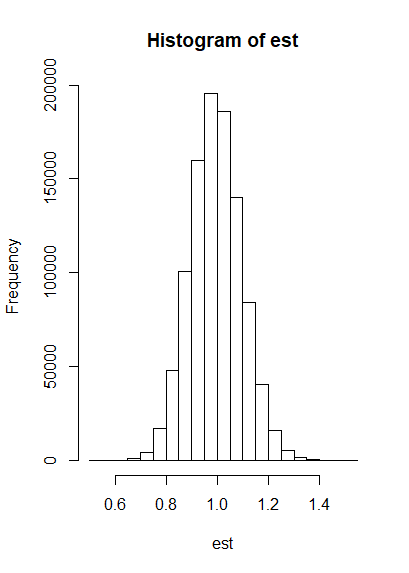
\includegraphics{Samplemeans.png}
		\end{figure}
	\item
		\begin{equation*}
		\begin{split}
		\sqrt{n}(\bar{X} - \lambda) &\rightarrow N(0,\sigma^{2}(x)) \\
		\sqrt{100}(\bar{X} - \lambda) &\rightarrow N(1,1) \\
		(\bar{X} - \lambda) &\rightarrow N(1,\frac{1}{100}) \\
		\end{split}
		\end{equation*}		
	\item
		$\bar{X}$ = 1.00004195 \\
		$\bar{X} - X \approx$ 0 \\
		$Var[X]$ = .009978 \\
		These match.
	\end{enumerate}
\item
	\begin{enumerate}
	\item
		It sure looks normal to me. It's even more symmetric than the last one with a similar quartile range. 
		\begin{figure}[H]
		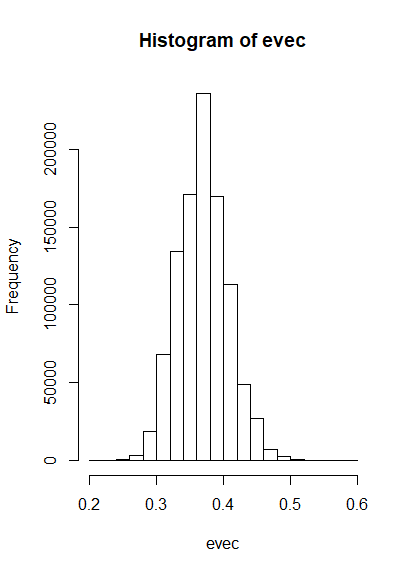
\includegraphics{evec.png}
		\end{figure}
	\item
		\begin{equation*}
		\begin{split}
		\sqrt{n}(\bar{X} - \lambda) &\rightarrow N(e^{-1},\sigma^{2}(x)\frac{d}{dx}(e^{-x})^{2}) \\
		(\bar{X} - \lambda) &\rightarrow N(e^{-1},\frac{1}{100}(-e^{-1})^{2}) \\
		(\bar{X} - \lambda) &\rightarrow N(e^{-1},\frac{e^{-2}}{100}) \\
		\end{split}
		\end{equation*}
	\item
		$\bar{X}$ = .369698 \\
		$\bar{X} - \lambda \approx$ 0 \\
		$Var[X]$ = .001357471 \\
		These match.
	\end{enumerate}
\end{enumerate}

\end{document}
